\documentclass[12pt]{article}

\usepackage[margin=1in]{geometry}
\usepackage[T1]{fontenc}
\usepackage{lmodern}
\usepackage{microtype}
\usepackage{amsmath,amssymb}
\usepackage{booktabs,threeparttable,longtable}
\usepackage{graphicx}
\usepackage[labelfont=bf]{caption}
\usepackage{setspace}
\usepackage[round,authoryear]{natbib}
\usepackage{xcolor}
\usepackage[colorlinks=true,linkcolor=blue!50!black,citecolor=blue!50!black,urlcolor=blue!50!black]{hyperref}

\onehalfspacing
\setlength{\parskip}{0pt}
\captionsetup{font=small}

\title{Do the Effects of State R\&D Tax Credits\\ Build Up over Time?\\[4pt]
\large Evidence from U.S.\ Patenting, 1976--2019}
\author{Bingrui Wang\thanks{New York University. Email: \href{mailto:bw3124@nyu.edu}{bw3124@nyu.edu}.
The code and data-construction scripts are available from the author.}}
\date{November 2026}

\begin{document}
\maketitle

\begin{abstract}
\noindent Between 1982 and 2012, 23 U.S.\ states in my sample introduced an R\&D tax credit and kept it in
place. I use the staggered timing of these adoptions to ask whether the credits raised patenting by inventors
in the adopting state, and whether any effect grew or faded the longer a credit stayed in force. Patents are
counted by inventor state and filing year from the full set of U.S.\ utility patents, and effects are estimated
with the event-study estimator of \citet{callaway2021difference}. I find no detectable effect at any horizon.
In the first three years after adoption, patenting is 3.5 log points higher than in the year before adoption
(s.e.\ 2.1), but it was 4.4 log points higher in the years before that as well. Measured against those earlier
years, the short-run effect is $-0.9$ log points (s.e.\ 2.9). Averaged over twenty years, the effect is $-3.8$
log points (s.e.\ 8.7), with no sign that effects build up. Splitting patents by the size of the owning
organization, or credits by their effective value, reveals no reliable differences. The results extend recent
evidence that state credits did not raise patent counts by showing that the null holds in the short run and in
the long run alike.

\medskip
\noindent\textbf{JEL codes:} H25, H71, O31, O38\\
\noindent\textbf{Keywords:} R\&D tax credits, innovation, patents, state tax policy, event study
\end{abstract}

\newpage

%==========================================================================
\section{Introduction}
%==========================================================================

By 2006, 32 U.S.\ states offered a general tax credit for company-funded research and development
\citep{wilson2009beggar}, and several more have created one since \citep{iowa2021research}. A large
literature finds that R\&D tax incentives raise measured R\&D spending
\citep{hall1993rd,hall2000effective,bloom2002credits,rao2016credits,guceri2019effectiveness}, and in a review
of innovation policies \citet{bloom2019toolkit} rank R\&D tax credits among the most effective tools in the
short run. Whether state credits raise innovation \emph{output} is less clear. Reported R\&D can rise because
firms relabel existing spending as research \citep{chen2021notching}, and a state's gain can come partly at the
expense of other states \citep{wilson2009beggar}. Using patents, \citet{melnik2024rd} find no aggregate
increase in patenting after states adopt credits, although the novelty and market value of patents rise.

This paper asks a narrower question about timing. An average effect close to zero can hide two quite
different patterns. A credit might raise patenting for a few years and then stop mattering, for example if
firms mainly move projects forward in time, or if the advantage over other states erodes as more states adopt.
Alternatively, effects might start small and build up, because R\&D adds to a stock of knowledge that keeps
producing inventions \citep{griliches1979issues} and because inventors move toward low-tax states only
gradually \citep{moretti2017effect}. The two patterns have different policy implications. A credit that only
shifts the timing of innovation is an expensive way to change little, while a credit whose effects build up
will look ineffective in short evaluations. Cross-sectional comparisons cannot separate these possibilities.
In my data, states with a credit in force have about three times as many patents per resident as states that
never adopted one, but the same states already had almost twice as many before they adopted (Table
\ref{tab:descriptives}).

I use the staggered adoption of state credits and follow patenting in each adopting state from ten years
before to twenty years after its credit started. The policy dates combine two sources, \citet{wilson2009beggar}
and \citet{iowa2021research}, and I keep only states whose dates agree within one year. Patents are every U.S.\
utility patent with at least one U.S.\ inventor, assigned to states by the inventors' locations and to years
by the filing date. The estimation sample contains 23 adopting states, which form 18 adoption cohorts between
1982 and 2012, and 9 states that never adopted a credit, observed from 1976 to 2019. Because adoption is
staggered and effects may change over time, I use the estimator of \citet{callaway2021difference}, which
compares each adoption cohort only with states that have not yet adopted, instead of a conventional two-way
fixed effects regression, whose estimates can be biased in this setting
\citep{goodmanbacon2021difference,roth2023trending}.

There are three findings. First, there is no short-run increase in patenting once the right comparison is
made. Relative to the year before adoption, patenting is 3.5 log points higher in the first three years
(s.e.\ 2.1). All nine pre-adoption estimates are positive as well, however, and patenting in years $-5$ to $-2$
is 4.4 log points (s.e.\ 2.3) above the year before adoption. The year before adoption is a low year, and
patenting after adoption returns to its earlier level rather than rising above it. Compared with years $-5$ to
$-2$, the short-run effect is $-0.9$ log points (s.e.\ 2.9), and the 95 percent confidence interval rules out
short-run increases larger than about 5 percent. Second, there is no sign that effects build up: the estimates
for years 3--10 and 11--20 are negative, though imprecise, and the twenty-year average is $-3.8$ log points
with a confidence interval from $-20.7$ to $13.2$. Third, the null holds for patents owned by small and by
large organizations and for credits of high and of low effective value. The estimates for small owners are
hard to interpret, because their patenting in adopting states was already falling relative to other states
before the credits started.

The paper contributes to the literature on state R\&D tax credits
\citep{wilson2009beggar,moretti2014state,chang2018endogeneity,melnik2024rd} by studying how effects on
innovation output evolve with the time since adoption. It complements firm-level evidence that more generous tax
relief raises the R\&D and patenting of the firms that receive it \citep{dechezlepretre2023tax} and that small firms respond
more in their R\&D spending \citep{agrawal2020small,rao2026tax}. The state-level null suggests that whatever
the credits do for some firms is too small, or too offset elsewhere, to show up in a state's patent count.
The paper also illustrates a practical point for event studies. When every estimate is measured against a
single base year, an unusually low base year makes the years after treatment look like an increase. This is a
version of the pre-program dip familiar from the evaluation of training programs \citep{ashenfelter1978estimating},
and it is visible only when the pre-treatment estimates are plotted on the same baseline as the post-treatment
ones \citep{roth2024interpreting}.

Section \ref{sec:background} describes the credits and the reasons their effects might build up or fade.
Section \ref{sec:data} describes the data, and Section \ref{sec:method} the estimators. Section
\ref{sec:results} presents the main results and robustness checks, Section \ref{sec:heterogeneity} the
heterogeneity by owner size and credit value, and Section \ref{sec:discussion} discusses interpretation and
limitations. Section \ref{sec:conclusion} concludes.

%==========================================================================
\section{Background}\label{sec:background}
%==========================================================================

\subsection{State R\&D tax credits}

The federal research credit was introduced in 1981 and lets firms subtract a share of their qualified research
spending above a base amount from their tax bill \citep{hall1993rd}. States soon added credits against their own
corporate income taxes; the earliest in \citeauthor{wilson2009beggar}'s (\citeyear{wilson2009beggar}) list is
Minnesota's, enacted in 1982. Most state credits follow the federal design: 19 of the 32 credits in Wilson's
list define the base as the federal credit does. They are incremental, so a firm earns the credit only on
research above a base, and the definition of the base matters a great deal for how much the credit is worth. When the base is a fixed historical ratio, as in the federal credit, a dollar of extra
research earns roughly the statutory rate. When the base is a moving average of the firm's own recent
research, extra research today raises the base in future years and claws back most of the credit. For this
reason \citet{wilson2009beggar} reports an effective rate of 0.5 percent for Illinois, whose statutory rate is
6.5 percent but whose base is the average of the previous three years, compared with 10 to 17 percent for
the fixed-base credits of Arizona, Massachusetts, New Jersey, and Rhode Island. \citet{rao2026tax} make the
same point about the federal credit: complex base rules push effective rates far below statutory rates and
can discourage research in later years.

Two features of state credits make them a useful setting for studying timing. First, adoption is staggered
over three decades (Figure \ref{fig:timeline}), so different states are observed at the same time since
adoption in different calendar years. Second, once adopted, most credits stayed in force. Among the 27 adopters in
my main sample, only four repealed their credit before 2020, and I drop them from the main estimates.

\subsection{Why effects might build up or fade}

Several mechanisms predict that effects on innovation grow over time. Research builds a stock of knowledge
that keeps producing inventions after the spending that created it \citep{griliches1979issues}, and the
returns to that stock are large \citep{hall2010measuring}. Firms adjust research budgets slowly: in the
federal credit's first decade, \citet{hall1993rd} finds that firms took several years to adjust fully and that
long-run effects were probably large, and \citet{bloom2002credits} estimate long-run responses of R\&D to its
tax price that are much larger than short-run ones. People also move slowly: the location of star scientists
responds to state taxes, and the response grows with time \citep{moretti2017effect}. If credits work through
these channels, a state's patenting should rise gradually after adoption.

Other mechanisms predict effects that are small from the start or that fade. If part of the measured R\&D
response is relabeling \citep{chen2021notching}, reported research rises without any change in invention. If
credits mainly attract research from other states \citep{wilson2009beggar,moretti2014state}, the advantage of
an early adopter should shrink as more states offer similar credits; this is my interpretation of their
findings rather than a result they test. Moving-average bases reduce the value of extra research in later
years, as described above. Finally, patents capture only part of innovation, and the share of inventions that
are patented differs across industries and over time \citep{griliches1990patent}.

\subsection{Why firm size might matter}

Research is hard to finance externally, because it produces intangible assets that make poor collateral and
because outsiders know less about a project than the firm does \citep{hall2010financing}. These frictions bind
more for small and young firms. \citet{brown2009financing} find that cash flow and new equity drive the R\&D of
young firms but not of mature ones, and \citet{howell2017financing} shows that early-stage R\&D grants help
small firms by easing their financing constraints. A tax credit adds cash flow, so it may matter most where
cash is scarce. Consistent with this, small firms raise R\&D more in response to tax incentives
\citep{agrawal2020small,castellacci2015meta,rao2026tax}, incentives are much less effective for large and
R\&D-intensive firms \citep{appelt2025effective}, and in the related setting of investment incentives small
firms respond far more than large ones \citep{zwick2017tax}. Small and large firms also produce different
kinds of innovation \citep{akcigit2018growth}.

There are also reasons to expect the opposite. Small firms often fail to claim tax benefits they are entitled
to \citep{zwick2021costs}, and a credit against income tax has no immediate value for a firm that makes losses
and owes no tax. Large firms produce most patents, and \citet{melnik2024rd} find that their results are driven
by larger firms.

%==========================================================================
\section{Data}\label{sec:data}
%==========================================================================

\subsection{Credit adoption dates}

I code the years in which each state offered a credit from two sources. \citet{wilson2009beggar} lists the 32
states with a general credit on company-funded R\&D as of 2006, with the year each was enacted and its
statutory and effective rates. \citet{iowa2021research} lists each state's current credit program with its
first tax year and, where relevant, its sunset year. I transcribe both by hand and apply five rules, all fixed
before estimation. (i) The start year is Wilson's enactment year for the 32 states in his table. (ii) For
credits created after 2006, which Wilson could not cover, the start year is Iowa's first tax year; in the main
sample these are Michigan, Virginia, and Florida. (iii) Six states appear in the Iowa list with a credit
starting in 2006 or earlier but are absent from Wilson's table, which covers only general credits. I treat
their absence as a sign that the credits are not standard and exclude all six; for three of them the Iowa list
itself notes a restriction (Colorado's credit is limited to enterprise zones, New Mexico's to firms with at most
50 employees, and Washington's is a credit against its business and occupation tax). (iv) The end year is Iowa's
sunset year if that year was 2020 or earlier. (v) I exclude states whose two sources disagree by more than one
year, which happens mostly because the Iowa list reports only a state's current program and misses earlier
ones, and New Hampshire, whose credit was switched off and on again. Table \ref{tab:policy} in the appendix
reports both sources and the coding for all 50 states and the District of Columbia.

Rule (ii) admits Florida even though the Iowa list notes that its credit
is limited to target industries. The rules leave 36 jurisdictions: 27 that adopted a credit and 9 that never did (Alabama, the District of
Columbia, Kentucky, Mississippi, Nevada, Oklahoma, South Dakota, Tennessee, and Wyoming). Four adopters
repealed their credit before 2020 (Michigan, Missouri, North Carolina, and Oregon). Because the event study
asks what happens in the years after a credit starts, I drop these four from the main estimates and add them
back in a robustness check. Figure \ref{fig:timeline} shows the timing for the remaining states. Two checks
compare the coding with what the sources themselves report. Under my coding, 31 of the 32 states in Wilson's
table have an active credit in 2006; the exception is Missouri, whose credit had expired according to the Iowa
list. Rebuilding Iowa's own count of states with a credit in each year from its program dates reproduces the
count in 27 of 41 years, and the differences arise because its program list omits credits that were later
replaced.

\begin{figure}[t]
\centering
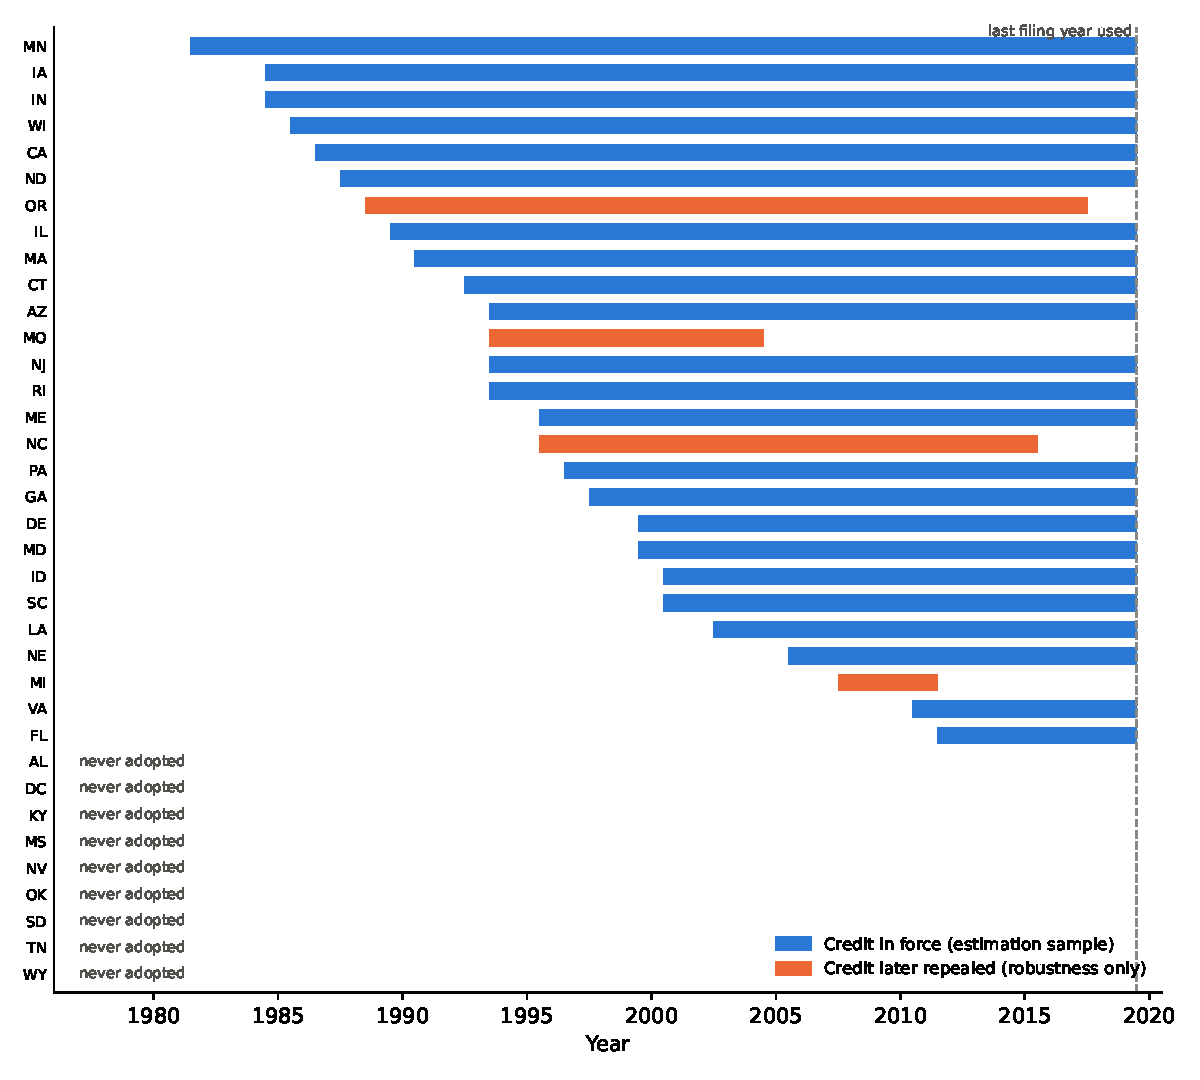
\includegraphics[width=0.78\textwidth]{figures/fig1_adoption_timeline.pdf}
\caption{Timing of state R\&D tax credits in the main sample}
\label{fig:timeline}
\caption*{\footnotesize \textit{Notes:} Each bar runs from the first year of a state's credit to 2019, the last
filing year used, or to the year the credit expired. The 23 states with blue bars and the 9 never-adopting
states form the estimation sample. The 4 states with orange bars repealed their credit and are used only in
a robustness check. Fifteen other states are excluded because their credit is non-standard or the sources
disagree about its timing (Table \ref{tab:policy}).}
\end{figure}

\subsection{Patents}

Patent data come from the USPTO's PatentsView database \citep{uspto2026patentsview}, which covers all patents
granted from 1976 to 2025 and links each inventor to a disambiguated location. I keep the 8.5 million utility
patents, take each patent's filing date from the application records, and assign it to states through its
inventors. A patent with $n$ inventors adds $1/n$ to the state of each inventor, so a patent with two inventors
in California and one in Texas adds two thirds to California and one third to Texas, and inventors outside the
United States reduce the share counted in any state. Fractional counting avoids counting a patent more than
once when its inventors live in different states.

I date patents by the filing year rather than the grant year, because the filing date is closer to when the
invention was made and the time from filing to grant has varied over time. Recent filing years are incomplete,
because many applications filed in those years were still pending when the data were released. This is the
usual truncation problem in patent data \citep{hall2001nber}, and I avoid it by using filing years up to 2019
only. As a check on the construction, I also count patents by grant year and compare the state totals with
the patent counts published by the National Center for Science and Engineering Statistics
\citep{ncses2026state}. Across 1,479 state-years the correlation is 1.000 and the ratio of the totals is 1.00.

\subsection{Patent owners and their size}

To split patents by the size of their owner, I use the first-listed assignee of each patent. If that assignee
is classified by the USPTO as a U.S.\ or foreign company or corporation, I measure its size by the total number
of U.S.\ utility patents it holds in the whole data. Owners with fewer than 50 patents are small, those with 50
to 499 are medium, and those with 500 or more are large; patents without an organizational owner, which are
held by individual inventors or governments, form a fourth group. The thresholds were fixed before looking at
any results. The largest owners are familiar firms (IBM, Samsung Display, Canon, Sony, and Fujitsu), and of the
roughly 444,000 organizations, 431,796 are small and 1,661 are large. Among patents with U.S.\ inventors filed
from 1976 to 2019, 19.7 percent belong to small owners, 15.6 percent to medium owners, 48.4 percent to large
owners, and 16.3 percent have no organizational owner. In every state and year the four groups add up exactly
to the total count.

The data contain no employment or sales, so patents stand in for firm size. Two limitations follow. A firm's
size is measured over the whole period, including years after the credits started, and the first-listed
assignee need not be located in the inventor's state. Section \ref{sec:heterogeneity} returns to both.

\subsection{Other data and descriptive statistics}

State population comes from the Bureau of Economic Analysis \citep{bea2026regional} and business-performed R\&D
from the NCSES State Indicators \citep{ncses2026state}. The R\&D series starts in 1997 and has some suppressed
values, which limits its use (Appendix \ref{app:rd}).

Table \ref{tab:descriptives} describes the estimation sample. Adopting states are larger and patent more per
resident than never-adopting states, both before adoption (20.4 patents per 100,000 residents) and after (35.7),
compared with 11.4 in never-adopting states. The patent counts are highly skewed: in 2015, inventors in California
filed about four times as many patents as inventors in Texas, the next state. This is why all outcomes are in logs and why one robustness check
drops California.

{\setlength{\tabcolsep}{4pt}\begin{table}[t]
\centering
\caption{Descriptive statistics, estimation sample, 1976--2019}
\label{tab:descriptives}
\begin{threeparttable}
\begin{tabular}{lccc}
\toprule
 & \multicolumn{2}{c}{Adopting states} & Never-adopting \\
\cmidrule(lr){2-3}
 & Before adoption & After adoption & states \\
\midrule
Patents per year (fractional count) & 1,077 & 3,122 & 304 \\
 & (1,126) & (6,003) & (263) \\[2pt]
Patents per 100,000 residents & 20.4 & 35.7 & 11.4 \\
 & (17.4) & (22.7) & (5.9) \\[2pt]
Population (millions) & 5.6 & 7.1 & 2.6 \\
 & (5.1) & (7.9) & (1.8) \\[2pt]
Business R\&D, \$ millions (1997--2019) & 2,341 & 8,318 & 653 \\
 & (1,804) & (17,882) & (592) \\[2pt]
Share of patents (\%) held by: & & & \\
\quad small owners ($<$50 patents) & 20.2 & 20.0 & 24.4 \\
\quad medium owners (50--499) & 14.0 & 17.0 & 15.5 \\
\quad large owners (500+) & 36.9 & 50.2 & 32.8 \\
\quad no organization owner & 28.9 & 12.8 & 27.3 \\
\midrule
States & 23 & 23 & 9 \\
State-years & 446 & 566 & 396 \\
\bottomrule
\end{tabular}
\begin{tablenotes}[flushleft]\footnotesize
\item \textit{Notes:} Means across state-years, standard deviations in parentheses. Patents are
utility patents counted by the filing year and divided equally among inventors, so a patent with
inventors in two states adds one half to each. Owner size is the number of patents the first-listed
organization owner holds in the whole data. Business R\&D comes from NCSES and starts in 1997;
some state-years are suppressed. The before and after columns contain the same 23 states.
\end{tablenotes}
\end{threeparttable}
\end{table}
}

%==========================================================================
\section{Empirical strategy}\label{sec:method}
%==========================================================================

Let $Y_{st}$ be the log of the fractional patent count of state $s$ in filing year $t$, and let $G_s$ be the
first year in which state $s$ has a credit, with $G_s = 0$ for states that never adopt. Event time
$e = t - G_s$ counts the years since adoption, so $e=0$ is the first year with a credit and $e=-1$ the year
before.

\paragraph{Two-way fixed effects.} The conventional event study regresses the outcome on event-time indicators
with state and year fixed effects:
\begin{equation}\label{eq:twfe}
Y_{st} = \alpha_s + \lambda_t + \sum_{k \neq -1} \beta_k \, \mathbf{1}\{t - G_s = k\} + \varepsilon_{st},
\end{equation}
where $k$ runs from $-10$ to $20$, the end points collect all earlier and later years, and the indicators are
zero for never-adopting states. Each $\beta_k$ measures the outcome $k$ years from adoption relative to the year
before adoption. With staggered adoption, however, equation \eqref{eq:twfe} uses states that adopted earlier as
comparisons for states that adopt later. If effects change with time since adoption, those comparisons are
contaminated, and the estimated $\beta_k$ need not equal a weighted average of the true effects
\citep{goodmanbacon2021difference,roth2023trending}. Because the question of this paper is precisely whether
effects change over time, this is the relevant concern.

\paragraph{Callaway and Sant'Anna.} The main estimates therefore use the estimator of
\citet{callaway2021difference}, which never uses already-treated states as comparisons. For each adoption
cohort $g$ and year $t$, it compares the change in the outcome since the year before adoption in that cohort
with the same change in states that have not adopted by year $t$:
\begin{equation}\label{eq:attgt}
\widehat{ATT}(g,t) = \Big(\bar Y_{g,t} - \bar Y_{g,g-1}\Big) - \Big(\bar Y_{C(g,t),t} - \bar Y_{C(g,t),g-1}\Big),
\end{equation}
where $\bar Y_{g,t}$ is the average outcome of the states in cohort $g$ in year $t$ and $C(g,t)$ contains the
never-adopting states and the states that adopt after both $t$ and $g-1$. The event-time effect $\theta(e)$
averages $\widehat{ATT}(g, g+e)$ across the cohorts observed $e$ years after adoption, weighting each cohort by
its number of states. For $e<0$ the same formula gives pre-adoption estimates. I measure them, like the
post-adoption estimates, against the year before adoption. \citet{roth2024interpreting} shows that the
alternative used by default in common software, which compares each pre-adoption year with the year just before
it, produces pre-period estimates that cannot be read the same way as the post-period ones. The choice does not
affect any post-adoption estimate. I use no covariates, and in a robustness check I restrict $C(g,t)$ to
never-adopting states.

To summarize the event study, I average $\theta(e)$ over four horizons: years 0--2, 3--10, 11--20, and 0--20.
The longer horizons rest on fewer cohorts: an effect twenty years after adoption is observed only for the 15
states that adopted by 1999, so the late horizons describe early adopters. Standard errors come from a
bootstrap that resamples the 32 states with replacement 999 times, keeping all years of a state together,
which clusters by state; each replication repeats the whole estimation. A joint test that the estimates for
years $-10$ to $-2$ are all zero uses the bootstrap covariance matrix.\footnote{I wrote the estimator for this
paper and checked it against the \texttt{csdid} package: for all 774 cohort-year cells, the group-time effects
agree to within $10^{-15}$ for both comparison groups and both choices of base year. An early version of the
Python package \texttt{moderndid} (0.0.3) agrees for never-adopting comparisons but returns different values,
and omits some cells, when the comparison group includes states that adopt later. Appendix \ref{app:check}
gives details.}

\paragraph{Identification.} The estimates have a causal interpretation if, absent the credit, patenting in
adopting states would have evolved like patenting in the comparison states, and if patenting did not respond
to a credit before it started. The first assumption fails if states adopt credits in response to the
trajectory of their own innovation. \citet{chang2018endogeneity} finds evidence that state R\&D credit policy is
endogenous to state economic conditions, so this is a real concern, and the pre-adoption estimates are the main evidence on
it. A second threat is other policies that change at the same time, such as corporate tax rates, which also
affect state innovation \citep{mukherjee2017taxes,akcigit2022taxation}. A third is spillovers: if a credit pulls
inventors from other states \citep{wilson2009beggar,moretti2014state}, the comparison states lose patents and the
estimates overstate the effect on total innovation. Since the estimates are close to zero, this last bias
would make the true effect on total patenting, if anything, smaller.

%==========================================================================
\section{Results}\label{sec:results}
%==========================================================================

\subsection{Patenting before and after adoption}

Figure \ref{fig:main} shows the event study for log patents. The two estimators give almost the same estimates,
which is expected when the effects are close to zero, since the bias of the two-way fixed effects estimator
comes from effects that differ across cohorts and over time. Before adoption, all nine estimates are positive
and stable at roughly 2 to 7 log points, and joint tests do not reject that they are zero
($p = 0.572$ for Callaway--Sant'Anna and $p = 0.153$ for two-way fixed effects). In the first three years after
adoption, the estimates are 4.7, 3.6, and 2.3 log points. From year 3 to year 19 they are negative, between
about $-1$ and $-11$ log points, with wide confidence intervals.

\begin{figure}[t]
\centering
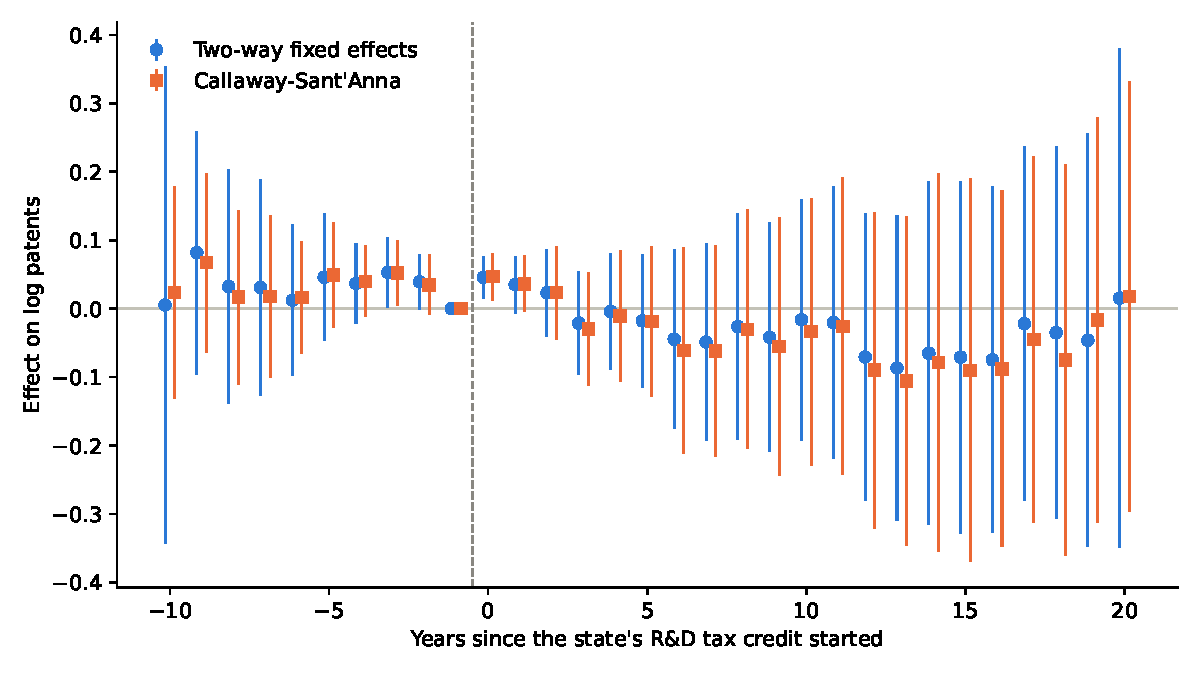
\includegraphics[width=0.95\textwidth]{figures/fig2_event_study_patents.pdf}
\caption{Log patents before and after a state adopts an R\&D tax credit}
\label{fig:main}
\caption*{\footnotesize \textit{Notes:} Estimates of the change in log patents (fractional count by inventor
state and filing year) relative to the year before adoption, for 23 adopting and 9 never-adopting states,
1976--2019. Callaway--Sant'Anna estimates compare each adoption cohort with states that have not yet adopted;
two-way fixed effects estimates come from equation \eqref{eq:twfe}, with the end points binned. Bars show 95
percent confidence intervals clustered by state.}
\end{figure}

{\setlength{\tabcolsep}{4pt}\begin{table}[t]
\centering
\caption{Effect of adopting an R\&D tax credit on log patents}
\label{tab:main}
\begin{threeparttable}
\begin{tabular}{lccc}
\toprule
 & (1) & (2) & (3) \\
 & CS, not-yet-treated & CS, never-treated & TWFE \\
 & comparison & comparison & event study \\
\midrule
Years 0--2 & $0.035^{*}$ & $0.048^{*}$ & $0.035^{*}$ \\
 & $(0.021)$ & $(0.027)$ & $(0.021)$ \\[2pt]
Years 3--10 & $-0.038$ & $-0.011$ & $-0.027$ \\
 & $(0.070)$ & $(0.070)$ & $(0.064)$ \\[2pt]
Years 11--20 & $-0.060$ & $-0.044$ & $-0.048$ \\
 & $(0.128)$ & $(0.140)$ & $(0.128)$ \\[2pt]
Years 0--20 (all) & $-0.038$ & $-0.018$ & $-0.028$ \\
 & $(0.087)$ & $(0.095)$ & $(0.086)$ \\[2pt]
\midrule
\multicolumn{4}{l}{\textit{Compared with the years before adoption}} \\
Years $-5$ to $-2$ (before adoption) & $0.044^{*}$ & $0.040$ & $0.044$ \\
 & $(0.023)$ & $(0.032)$ & $(0.027)$ \\[2pt]
Years 0--2 minus years $-5$ to $-2$ & $-0.009$ & $0.007$ & $-0.009$ \\
 & $(0.029)$ & $(0.044)$ & $(0.036)$ \\[2pt]
\midrule
Pre-trend test, $p$-value & 0.572 & 0.473 & 0.153 \\
\midrule
Adopting / never-adopting states & 23 / 9 & 23 / 9 & 23 / 9 \\
State-years & 1,408 & 1,408 & 1,408 \\
\bottomrule
\end{tabular}
\begin{tablenotes}[flushleft]\footnotesize
\item \textit{Notes:} Each entry averages the event-time estimates over the years shown; year 0 is
the first year with a credit. All estimates measure log patents relative to the year before adoption
(year $-1$), except the last estimate row, which compares years 0--2 with the average of years $-5$ to $-2$.
Columns (1) and (2) use the estimator of \citet{callaway2021difference}; column (1) compares each
adoption cohort with states that never adopt or adopt later, column (2) with never-adopting states only.
Column (3) regresses log patents on event-time indicators with state and year fixed effects (endpoints
binned at $-10$ and $+20$). Standard errors clustered by state: bootstrap with 999 state resamples in
(1)--(2), analytic in (3). The pre-trend test asks whether the estimates for years $-10$ to $-2$ are jointly
zero. $^{*}p<0.1$, $^{**}p<0.05$, $^{***}p<0.01$.
\end{tablenotes}
\end{threeparttable}
\end{table}
}

Table \ref{tab:main} summarizes the figure. In column (1), patenting in years 0--2 is 3.5 log points higher than in
the year before adoption (s.e.\ 2.1, $p = 0.10$). Taken alone, this looks like a modest short-run increase. The
pre-adoption estimates show why it is not. Patenting in years $-5$ to $-2$ is also 4.4 log points above the year
before adoption (s.e.\ 2.3). The year before adoption is therefore a low year, and after adoption patenting simply
returns to the level of the earlier years. When the post-adoption years are compared with years $-5$ to $-2$
instead of with year $-1$ alone, the short-run effect is $-0.9$ log points (s.e.\ 2.9). Its 95 percent confidence
interval runs from $-6.6$ to $4.8$ log points, so the data rule out short-run increases larger than about 5
percent. The joint pre-trend tests do not detect this pattern because the pre-adoption estimates are level rather
than trending; the problem is the base year, not a diverging trend.

Two explanations for the low year before adoption fit the data, and I cannot distinguish them. States may adopt
credits after a weak year for innovation, the policy analogue of the dip in earnings before workers enter training
programs \citep{ashenfelter1978estimating}; this would be consistent with the policy endogeneity documented by
\citet{chang2018endogeneity}. Alternatively, firms that expect a credit may postpone research or filings until it
is available, which moves patents from the year before adoption to the years after without adding to them. Under
either explanation, the year before adoption is a poor baseline and the comparison with earlier years is the
relevant one. Neither explanation implies that the credits raised patenting.

\subsection{Do effects build up?}

The estimates for later horizons give no sign that effects build up with time. Averaged over years 3--10, the
effect is $-3.8$ log points (s.e.\ 7.0), and over years 11--20 it is $-6.0$ log points (s.e.\ 12.8). The average
over all twenty years is $-3.8$ log points (s.e.\ 8.7), with a 95 percent confidence interval from $-20.7$ to
$13.2$. These long-run estimates are imprecise: they cannot rule out moderate effects in either direction, and
they rest increasingly on the early adopters. What they do rule out is the pattern that motivated the question,
a small initial effect that grows into a large one. If the credits' effects had accumulated to, say, 20 percent
more patents after a decade, the estimates for years 11--20 would lie well above zero rather than below it.

The answer to the original question about policy duration is therefore negative. States that have offered
a credit for longer do patent more (Table \ref{tab:descriptives}), but within states, patenting does not rise
with the number of years a credit has been in force.

\subsection{Robustness}

Table \ref{tab:robustness} changes one choice at a time. Keeping the four states that later repealed their
credit, using Iowa's start years for the four states where the two sources differ by one year, comparing only
with never-adopting states, measuring patents per resident, or dropping California all leave the conclusions
unchanged. Across these specifications, the estimate for years 0--2 measured against the year before adoption
ranges from 2.4 to 4.8 log points, the twenty-year average ranges from $-5.8$ to $-1.1$ log points, and no
pre-trend test rejects at conventional levels. Because every row measures effects against the year before
adoption, its short-run estimate should be read with the same caution as column (1) of Table \ref{tab:main}.

{\setlength{\tabcolsep}{3pt}\begin{table}[t]
\centering
\caption{Robustness of the patent estimates}
\label{tab:robustness}
\small
\begin{threeparttable}
\begin{tabular}{lcr@{\,}lr@{\,}lc}
\toprule
 & States & \multicolumn{2}{c}{Years 0--2} & \multicolumn{2}{c}{Years 0--20} & Pre-trend \\
 & (adopt / never) & \multicolumn{2}{c}{} & \multicolumn{2}{c}{} & $p$-value \\
\midrule
Main specification & 23 / 9 & $0.035^{*}$ & $(0.021)$ & $-0.038$ & $(0.087)$ & 0.572 \\
Keep 4 states that later repealed & 27 / 9 & $0.030$ & $(0.020)$ & $-0.011$ & $(0.080)$ & 0.422 \\
Iowa start years for AZ, CA, IN, MN & 23 / 9 & $0.024$ & $(0.021)$ & $-0.046$ & $(0.088)$ & 0.575 \\
Never-adopting comparison only & 23 / 9 & $0.048^{*}$ & $(0.027)$ & $-0.018$ & $(0.095)$ & 0.473 \\
Log patents per 100,000 residents & 23 / 9 & $0.040^{*}$ & $(0.021)$ & $-0.013$ & $(0.081)$ & 0.594 \\
Drop California & 22 / 9 & $0.037^{*}$ & $(0.022)$ & $-0.058$ & $(0.086)$ & 0.582 \\
\bottomrule
\end{tabular}
\begin{tablenotes}[flushleft]\footnotesize
\item \textit{Notes:} Each row changes one choice from the main specification and re-estimates the
Callaway--Sant'Anna event study. Entries are average effects on log patents relative to the year before
adoption, with bootstrap standard errors clustered by state (999 resamples) in parentheses.
The main specification is column (1) of Table 2. Arizona, California, Indiana and Minnesota are the four
states whose two sources differ by one year. $^{*}p<0.1$, $^{**}p<0.05$, $^{***}p<0.01$.
\end{tablenotes}
\end{threeparttable}
\end{table}
}

Business R\&D spending would be a natural intermediate outcome, but the NCSES series begins in 1997. Only 8
adopting states adopted after that year and have complete data, and the pre-trend test rejects strongly. Table
\ref{tab:rd} in the appendix reports the estimates for completeness; they are close to zero and very imprecise,
and I do not draw conclusions from them.

%==========================================================================
\section{Heterogeneity}\label{sec:heterogeneity}
%==========================================================================

\subsection{Small and large patent owners}

Figure \ref{fig:size} and Panel A of Table \ref{tab:heterogeneity} repeat the analysis separately for patents owned
by small and by large organizations. Because small groups in small states can have years without patents, the
outcome is $\log(1+\text{patents})$. For years 0--2, the estimate is 4.8 log points for small owners (s.e.\ 4.8)
and $-4.0$ log points for large owners (s.e.\ 5.5). To test whether the two differ, I estimate the event study on
the difference $\log(1+\text{small}) - \log(1+\text{large})$, which uses the fact that both series come from the
same states. The difference is 8.8 log points (s.e.\ 7.7, $p = 0.25$) in years 0--2 and 8.8 log points
(s.e.\ 14.9) over twenty years. The data therefore give no evidence that the credits helped small owners more.

\begin{figure}[t]
\centering
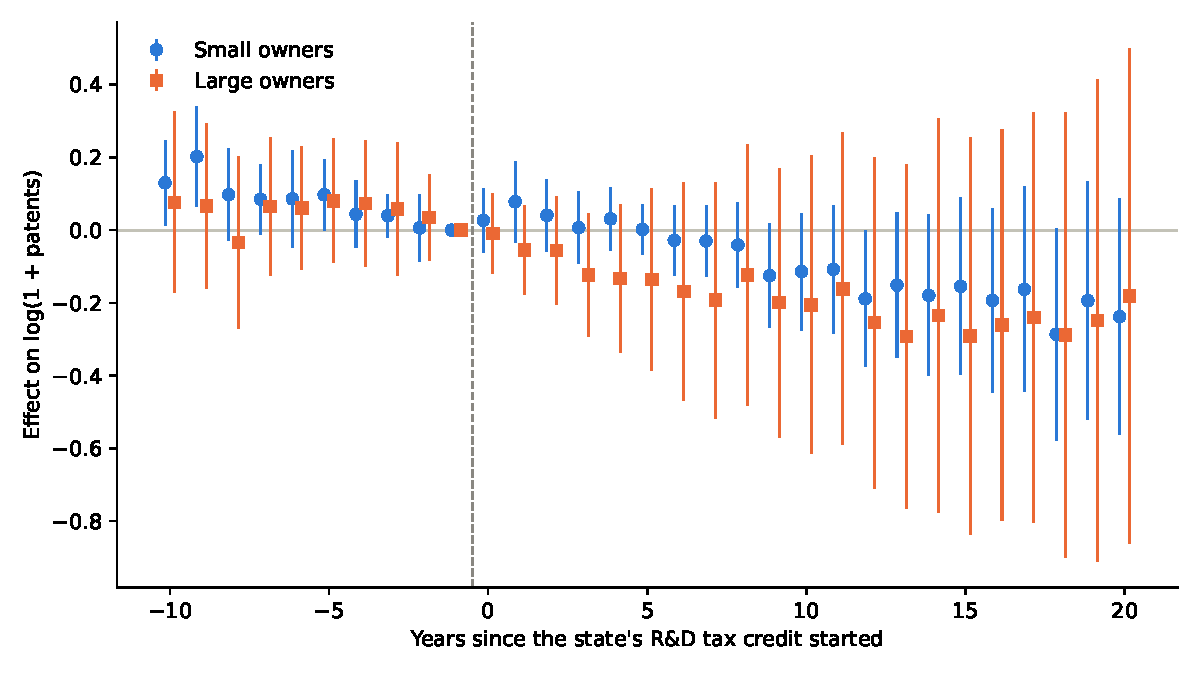
\includegraphics[width=0.95\textwidth]{figures/fig3_event_study_by_size.pdf}
\caption{Patents by size of the owning organization}
\label{fig:size}
\caption*{\footnotesize \textit{Notes:} Callaway--Sant'Anna estimates of the change in $\log(1+\text{patents})$
relative to the year before adoption, separately for patents whose first-listed owner holds fewer than 50 patents
(small) and 500 or more (large). Same sample as Figure \ref{fig:main}. Bars show 95 percent confidence intervals
clustered by state.}
\end{figure}

The small-owner series also shows why its estimates should not be read causally. Its pre-trend test rejects
($p = 0.004$): in adopting states, patenting by small owners declines relative to comparison states throughout
the ten years before adoption, and the decline continues at a similar pace afterwards (Figure
\ref{fig:size}). A steady relative decline that starts long before the credits is a trend, not a response to
them. The large-owner series has no such pre-trend ($p = 0.822$), but its post-adoption estimates are very
imprecise. Patents without an organizational owner, mostly those of individual inventors, show a small and
insignificant short-run estimate (3.2 log points, s.e.\ 2.4) and a decline over twenty years ($-10.6$ log points,
s.e.\ 5.4). This is the only estimate in Table \ref{tab:heterogeneity} that is significant even at the
10 percent level, and with this many outcomes one such estimate is not surprising, so I give it little weight.

These results differ in emphasis from \citet{melnik2024rd}, who find that their effects on patent value and
novelty come from larger firms. The difference is not necessarily a contradiction: their outcomes measure
the quality of patents, mine their number, and with patent counts large firms dominate any state total. The
measurement of size matters too. Because an owner's size is measured over the whole period, a small firm that
grew because of a credit would be classified as large, and because the first-listed owner may be located
elsewhere, a large out-of-state firm with a research lab in the state counts as large there. Both features blur
the comparison, but neither would hide a large difference.

\subsection{High-value and low-value credits}

If credits had any effect, it should be larger where they are worth more. Panel B of Table
\ref{tab:heterogeneity} splits the adopting states by the effective rate that \citet{wilson2009beggar} computes
for each credit. The six credits with a moving-average base have effective rates below 1 percent; the other 15
have rates between 2.5 and 16.9 percent. Each adoption cohort falls entirely into one group, so I average the
cohort effects separately for each group while keeping all states as potential comparisons. In years 0--2, the
estimate is 2.3 log points for high-value credits (s.e.\ 2.5) and 4.4 log points for low-value credits
(s.e.\ 4.2), a difference of $-2.1$ log points (s.e.\ 4.5). Over twenty years the estimates are $-2.9$ and $-8.1$
log points, both imprecise. If anything, the short-run estimate is smaller for the credits that are worth more,
which is hard to square with a causal effect of the credit and easy to square with the base-year pattern
described above.

\begin{table}[t]
\centering
\caption{Heterogeneity: owner size and credit value}
\label{tab:heterogeneity}
\begin{threeparttable}
\begin{tabular}{lr@{\,}lr@{\,}lc}
\toprule
 & \multicolumn{2}{c}{Years 0--2} & \multicolumn{2}{c}{Years 0--20} & Pre-trend $p$ \\
\midrule
\multicolumn{6}{l}{\textit{A. By size of the patent owner; outcome $\log(1+\text{patents})$}} \\
\quad Small owners ($<$50 patents) & $0.048$ & $(0.048)$ & $-0.096$ & $(0.080)$ & 0.004 \\
\quad Large owners (500+) & $-0.040$ & $(0.055)$ & $-0.184$ & $(0.183)$ & 0.822 \\
\quad No organization owner & $0.032$ & $(0.024)$ & $-0.106^{*}$ & $(0.054)$ & 0.792 \\
\quad Small minus large & $0.088$ & $(0.077)$ & $0.088$ & $(0.149)$ & 0.112 \\
\midrule
\multicolumn{6}{l}{\textit{B. By effective value of the credit; outcome log patents}} \\
\quad High-value credits (15 states) & $0.023$ & $(0.025)$ & $-0.029$ & $(0.099)$ & 0.647 \\
\quad Low-value credits (6 states) & $0.044$ & $(0.042)$ & $-0.081$ & $(0.117)$ & 0.057 \\
\quad High minus low & $-0.021$ & $(0.045)$ & $0.052$ & $(0.121)$ & \\
\bottomrule
\end{tabular}
\begin{tablenotes}[flushleft]\footnotesize
\item \textit{Notes:} Callaway--Sant'Anna estimates, not-yet-treated comparison, 23 adopting and 9
never-adopting states, 1976--2019. Panel A splits each state's patents by the size of the first-listed
organization owner (its total patents in the whole data); the difference row re-estimates the model on
the gap $\log(1+\text{small})-\log(1+\text{large})$. Panel B averages only the adoption cohorts whose
credit has a low effective rate (below 1 percent; all have a moving-average base: DE, IL, MD, ME, NE, PA)
or a high one (2.5 percent or more: AZ, CA, CT, GA, IA, ID, IN, LA, MA, MN, ND, NJ, RI, SC, WI), using the effective rates in
\citet{wilson2009beggar}; all states still serve as comparisons while they have not adopted.
Bootstrap standard errors clustered by state in parentheses. $^{*}p<0.1$, $^{**}p<0.05$, $^{***}p<0.01$.
\end{tablenotes}
\end{threeparttable}
\end{table}


%==========================================================================
\section{Discussion}\label{sec:discussion}
%==========================================================================

\paragraph{How large an effect can the data rule out?} The short-run confidence interval excludes increases in
patenting above about 5 percent. To put this in perspective, a credit with an effective rate of 5 to 10 percent
lowers the cost of a marginal research dollar by that amount. With user-cost elasticities of one or somewhat more, as
found in the R\&D literature \citep{hall1993rd,guceri2019effectiveness}, research would rise by a similar or
somewhat larger percentage,
and patents by less if patenting rises less than proportionally with research. Effects of that size are at the
edge of what the short-run estimates can detect. The results therefore rule out large short-run effects on
patent counts and any substantial build-up over time, but they cannot rule out small effects of the size the
R\&D literature would predict. The long-run estimates are much less precise.

\paragraph{Why might patent counts not respond?} The literature offers several reasons, which this paper cannot
separate. Many credits are worth little at the margin because of their base rules
\citep{wilson2009beggar,rao2026tax}. Part of the measured R\&D response elsewhere reflects relabeling
\citep{chen2021notching}, which changes tax filings but not inventions. Credits may change which projects firms
pursue rather than how many patents they file: \citet{melnik2024rd} find that patent novelty and value rise
even though counts do not. Finally, if the credits mainly moved research across state lines
\citep{wilson2009beggar,moretti2014state}, patents counted by inventor location would have risen in adopting
states even with no gain in total innovation. That they did not suggests that, for the average adopting state,
neither new nor relocated research was large enough to change the state's patent count.

\paragraph{Limitations.} Four limitations deserve mention. First, the policy coding treats adoption as a single
event and ignores changes in credit rates after adoption. Fifteen states are excluded because their credits are
non-standard or the sources disagree, and verifying their histories from state statutes would enlarge the
sample. Second, patent counts weight every patent equally and miss innovation that is not patented
\citep{griliches1990patent}; citation-weighted counts or measures of patent value would speak to quality.
Third, firm size is measured by patents and over the whole period. Firm-level data on employment and on the
location of research would allow a cleaner split. Fourth, with 32 states the long-run estimates are imprecise.
Sensitivity analysis that allows limited violations of parallel trends \citep{rambachan2023credible} would
show how robust the short-run conclusion is to the pre-adoption pattern; I leave it for future work.

%==========================================================================
\section{Conclusion}\label{sec:conclusion}
%==========================================================================

This paper asks whether state R\&D tax credits raised patenting in the states that adopted them, and whether
any effect grew or faded with the time since adoption. Using the staggered adoption of credits in 23 states and
an estimator that is robust to effects that change over time, I find no detectable effect at any horizon.
An apparent short-run increase of 3.5 log points disappears once patenting after adoption is compared with the
years before adoption rather than with the single low year just before it, and the estimates for later years give
no sign that effects build up. The null result holds for patents of small and large owners and for credits of
high and low effective value.

For policy, the results suggest that the innovation benefits of state credits, if any, are too small to show up in
patent counts, either right away or after twenty years. For empirical work, they show that the base period of an
event study deserves as much attention as the estimator: a single low year before treatment can produce an
apparent short-run effect.

\newpage
\bibliographystyle{plainnat}
\bibliography{references}

%==========================================================================
\newpage
\appendix
\setcounter{table}{0}
\setcounter{figure}{0}
\renewcommand{\thetable}{A\arabic{table}}
\renewcommand{\thefigure}{A\arabic{figure}}
\section{Credit coding for all states}\label{app:policy}
%==========================================================================

{\footnotesize
\setlength{\tabcolsep}{3pt}
\begin{longtable}{lccccccl}
\caption{State R\&D tax credits: sources and coding}\label{tab:policy}\\
\toprule
 & \multicolumn{2}{c}{Wilson (2009)} & \multicolumn{2}{c}{Iowa DOR (2021)} & \multicolumn{2}{c}{Used here} & \\
\cmidrule(lr){2-3}\cmidrule(lr){4-5}\cmidrule(lr){6-7}
State & Enacted & Eff.\ rate & First year & Sunset & Start & End & Status \\
\midrule
\endfirsthead
\toprule
State & Enacted & Eff.\ rate & First year & Sunset & Start & End & Status \\
\midrule
\endhead
Alabama &  &  &  &  &  &  & Never adopted \\
Alaska &  &  & 1998 &  &  &  & Excluded: non-standard credit \\
Arizona & 1994 & 11.0 & 1993 & 2030 & 1994 &  & Adopted \\
Arkansas &  &  & 2003 &  &  &  & Excluded: non-standard credit \\
California & 1987 & 13.7 & 1988 &  & 1987 &  & Adopted \\
Colorado &  &  & 1989 &  &  &  & Excluded: non-standard credit \\
Connecticut & 1993 & 6.0 & 1993 &  & 1993 &  & Adopted \\
Delaware & 2000 & 0.9 & 2000 &  & 2000 &  & Adopted \\
District of Columbia &  &  &  &  &  &  & Never adopted \\
Florida &  &  & 2012 &  & 2012 &  & Adopted \\
Georgia & 1998 & 10.0 & 1998 &  & 1998 &  & Adopted \\
Hawaii & 2000 & 20.0 & 2013 & 2024 &  &  & Excluded: sources disagree \\
Idaho & 2001 & 5.0 & 2001 &  & 2001 &  & Adopted \\
Illinois & 1990 & 0.5 & 1990 & 2027 & 1990 &  & Adopted \\
Indiana & 1985 & 5.0 & 1984 &  & 1985 &  & Adopted \\
Iowa & 1985 & 6.5 & 1985 &  & 1985 &  & Adopted \\
Kansas & 1988 & 0.4 & 2001 &  &  &  & Excluded: sources disagree \\
Kentucky &  &  &  &  &  &  & Never adopted \\
Louisiana & 2003 & 8.0 & 2003 &  & 2003 &  & Adopted \\
Maine & 1996 & 0.4 & 1996 &  & 1996 &  & Adopted \\
Maryland & 2000 & 0.9 & 2000 & 2027 & 2000 &  & Adopted \\
Massachusetts & 1991 & 10.0 & 1991 &  & 1991 &  & Adopted \\
Michigan &  &  & 2008 & 2011 & 2008 & 2011 & Adopted, later repealed \\
Minnesota & 1982 & 2.5 & 1981 &  & 1982 &  & Adopted \\
Mississippi &  &  &  &  &  &  & Never adopted \\
Missouri & 1994 & 0.5 & 1994 & 2004 & 1994 & 2004 & Adopted, later repealed \\
Montana & 1999 & 5.0 & 1987 & 2010 &  &  & Excluded: sources disagree \\
Nebraska & 2006 & 0.2 & 2006 & 2022 & 2006 &  & Adopted \\
Nevada &  &  &  &  &  &  & Never adopted \\
New Hampshire &  &  & 2007 &  &  &  & Excluded: credit off and on \\
New Jersey & 1994 & 10.0 & 1994 &  & 1994 &  & Adopted \\
New Mexico &  &  & 2000 &  &  &  & Excluded: non-standard credit \\
New York &  &  & 2005 &  &  &  & Excluded: non-standard credit \\
North Carolina & 1996 & 5.0 & 1996 & 2015 & 1996 & 2015 & Adopted, later repealed \\
North Dakota & 1988 & 4.0 & 1988 &  & 1988 &  & Adopted \\
Ohio & 2004 & 0.5 & 2001 &  &  &  & Excluded: sources disagree \\
Oklahoma &  &  &  &  &  &  & Never adopted \\
Oregon & 1989 & 5.0 & 1989 & 2017 & 1989 & 2017 & Adopted, later repealed \\
Pennsylvania & 1997 & 0.9 & 1997 &  & 1997 &  & Adopted \\
Rhode Island & 1994 & 16.9 & 1994 &  & 1994 &  & Adopted \\
South Carolina & 2001 & 5.0 & 2001 &  & 2001 &  & Adopted \\
South Dakota &  &  &  &  &  &  & Never adopted \\
Tennessee &  &  &  &  &  &  & Never adopted \\
Texas & 2001 & 5.0 & 2014 & 2026 &  &  & Excluded: sources disagree \\
Utah & 1999 & 6.0 & 2008 &  &  &  & Excluded: sources disagree \\
Vermont & 2003 & 0.9 & 2011 &  &  &  & Excluded: sources disagree \\
Virginia &  &  & 2011 & 2021 & 2011 &  & Adopted \\
Washington &  &  & 1995 & 2014 &  &  & Excluded: non-standard credit \\
West Virginia & 1986 & 10.0 & 2003 & 2012 &  &  & Excluded: sources disagree \\
Wisconsin & 1986 & 4.6 & 1986 &  & 1986 &  & Adopted \\
Wyoming &  &  &  &  &  &  & Never adopted \\
\bottomrule
\multicolumn{8}{p{0.95\textwidth}}{\footnotesize \textit{Notes:} Wilson (2009) lists the 32 states with a
general credit on company-funded R\&D as of 2006, with the year enacted and the effective credit rate
(percent). Iowa Department of Revenue (2021) lists each state's current program with its first tax year and
sunset year. The start year is Wilson's year where available and Iowa's year for credits created after
2006; the end year is an Iowa sunset that had already passed by 2020. States are excluded when Iowa
shows a pre-2006 credit that Wilson, who covers only general credits, leaves out,
when the two sources differ by more than one year, or when the credit was switched off and on.}\\
\end{longtable}

}

%==========================================================================
\section{Business R\&D spending}\label{app:rd}
%==========================================================================

Business-performed R\&D by state comes from the NCSES State Indicators, which start in 1997. Summed across
states, the 2019 values account for 99.8 percent of the national total; the remainder is suppressed or not
assigned to a state. Because the series starts in 1997, states that adopted earlier have no pre-adoption years
and cannot contribute, and states with any suppressed year drop out of the balanced panel. The resulting sample
has 8 adopting and 8 never-adopting states, and the pre-trend test rejects. Table \ref{tab:rd} reports the
estimates.

\begin{table}[t]
\centering
\caption{Business R\&D spending (appendix)}
\label{tab:rd}
\begin{threeparttable}
\begin{tabular}{lcc}
\toprule
 & CS, not-yet-treated & TWFE \\
\midrule
Years 0--2 & $0.013$ & $0.011$ \\
 & $(0.095)$ & $(0.083)$ \\[2pt]
Years 0--20 & $-0.023$ & $-0.020$ \\
 & $(0.138)$ & $(0.122)$ \\[2pt]
Pre-trend test, $p$-value & 0.000 & 0.000 \\
\midrule
Adopting / never-adopting states & 8 / 8 & 8 / 8 \\
State-years & 432 & 432 \\
\bottomrule
\end{tabular}
\begin{tablenotes}[flushleft]\footnotesize
\item \textit{Notes:} Outcome: log business-performed R\&D (NCSES), 1997--2023. Only states that adopted
after 1997 and have no suppressed years can contribute, which leaves few states, and the pre-trend test
rejects. These estimates are reported for completeness and are not used for inference in the text.
\end{tablenotes}
\end{threeparttable}
\end{table}


%==========================================================================
\section{Checking the estimator}\label{app:check}
%==========================================================================

The Callaway--Sant'Anna estimates in this paper come from code written for the project, which implements
equation \eqref{eq:attgt} and the aggregation described in Section \ref{sec:method} directly. To check it, I
compare every group-time effect for log patents with the \texttt{csdid} package, a Python port of the authors'
implementation. For each of the four combinations of comparison group (not-yet-treated or never-treated) and
base year (the year before adoption, or the previous year), all 774 cohort-year cells agree to within $10^{-15}$.

The first version of the analysis used the \texttt{moderndid} package (version 0.0.3). Its estimates agree with
both \texttt{csdid} and the code used here when the comparison group is never-adopting states, and on the
package's own example data they match a direct calculation from equation \eqref{eq:attgt}. When the
comparison group also includes states that adopt later, however, its estimates differ by up to 1.1 log points
in individual cells, and 35 of the 774 cells are missing. All estimates in this paper use the checked code.

\end{document}
